% This is samplepaper.tex, a sample chapter demonstrating the
% LLNCS macro package for Springer Computer Science proceedings;
% Version 2.20 of 2017/10/04
%
\documentclass[runningheads]{llncs}
%

\usepackage{caption}
\usepackage{graphicx}
% Used for displaying a sample figure. If possible, figure files should
% be included in EPS format.
%
% If you use the hyperref package, please uncomment the following line
% to display URLs in blue roman font according to Springer's eBook style:
% \renewcommand\UrlFont{\color{blue}\rmfamily}

\begin{document}
%
\title{Semi-supervised Learning using Variational Autoencoder - A Cluster based Approach}
%
%\titlerunning{Abbreviated paper title}
% If the paper title is too long for the running head, you can set
% an abbreviated paper title here
%
\author{Sunil Kumar Vengalil\inst{1}\orcidID{0000-1111-2222-3333} \and
Neelam Sinha\inst{1}\orcidID{1111-2222-3333-4444} }
%
\authorrunning{S. Vengalil et al.}
% First names are abbreviated in the running head.
% If there are more than two authors, 'et al.' is used.
%
\institute{International Institute of Information Technology, Bangalore, India\\
\url{https://www.iiitb.ac.in/} }
%
\maketitle              % typeset the header of the contribution
%
\begin{abstract}
The abstract should briefly summarize the contents of the paper in
150--250 words.

\keywords{Semi-supervised Learning  \and Variational Autoencoder \and Active Learning \and Clustering}
\end{abstract}
%
%
%
\section{Introduction}
Deep neural networks have been successfully applied in almost all domains for performing machine learning tasks like classification\cite{alexnet,vggnet,resnet}, object detection\cite{faster_rcnn,yolo} and segmentation\cite{deeplab,unet} in images and videos.
Recently, multi-layer deep neural networks have been identified as  effective  choices for  generative models also, Variational Autoencoder(VAE)\cite{vae} and Generative Adversarial networks(GAN)\cite{gan} being the most common examples.
One of the key tenets on which all these models work is  based upon  is the ability to learn a complex, parameterized unknown function using back propagation.
When trained with a huge amount of data for long enough durations and with appropriate regularization techniques, these networks are capable of learning functions that generalize well.
However, all these  models suffer from the following drawbacks
\begin{enumerate}
  \item Lack of explainability
  \item Need for huge amount of labelled data for supervised tasks like classification, object detection and segmentation
  \item Need for large computing power to train complex models with billions of parameters
\end{enumerate}

In this work, our key focus is on how to train a neural network faster, and with less number of annotated samples, by augmenting the training process with human feedback at regular intervals.
Instead of annotating all individual samples in the training set, we propose a mechanism where only a few representative samples (10-100) are annotated and the label of these samples are propagated to other training samples  which are closer to the labelled sample in the latent space.
It is very common to use  generative models, like Variational Autoencoder(VAE) \cite{vae} and Generative Adversarial Networks \cite{gan} in order to learn a low dimensional latent representation of data.
It is reasonable to assume, as validated correctly in our experimental results, that the samples which are closer in latent space have the same label.
In this work, we augment a popular generative model, variational autoencoder,  by adding a classification loss so that the latent space representations of samples from different classes becomes more separable.

Our work can also be looked at  as a novel  active learning framework using deep neural networks.
Active learning algorithms iteratively select ( or generate) samples for labelling which are used to improve the model performance.
The goal is to obtain sufficiently good performance of the trained model using as few labelled samples as possible.

We compare the results with different clustering algorithms k-means and Gaussian Mixture Model and also different distance metrics Mahalanobis vs Euclidean distance.

The major contributions of this paper are
\begin{enumerate}
    \item We propose a novel active learning framework where a  deep learning model incrementally learns to perform a task like image classification, while at the same time learning a low dimensional representation for the input data.
    \item We show that compared to existing deep active learning frameworks our approach requires very less number of training samples and also learns a latent representation and  probability distribution in the latent space from which new data samples can be drawn easily.
    \item Our experiments show that the distribution of latent vectors becomes multi-modal, and the multiple modes become more separable with the addition of a classification loss to the $\beta$-VAE loss function\cite{beta_vae}.
\end{enumerate}

\section{Related Work}
We are not the first to propose active learning using deep generative modelling.
Many of the existing work on active learning is based on either query-synthesizing or  pool-based methods.

Where as in query synthesizing new informative samples are generated using generative models, pool-based methods\cite{wang_2016,beluch_2018} depend on devising a smarter sampling strategy that can select a set of samples for labelling from the unlabelled data pool.
Many query-synthesizing methods use adversarial networks\cite{mahapatra_2018,mayer_2020} to generate new samples for labelling.
Our method is a combination of both query synthesizing and pool-based approach as we are generating new representative samples using clustering while at the same time selecting unlabelled samples from selected bad performing clusters.
In their work, Samarth et. al.\cite{vaal} uses Variational Autoencoder to learn a latent space along with an adversarial network to select samples for labelling from an unlabelled pool.

Our generative model is similar to the model described in\cite{kingma_2014}.
In \cite{kingma_2014}, a low dimensional embedding of unlabelled data is learned using a deep generative model.
The parameters of the generative model are optimized using variational lower bound and then the latent vectors in lower dimension are classified using SVM.
However, our work differs from \cite{kingma_2014} in respect that we introduce a novel mechanism for labelling by clustering the latent vectors.

\section{Proposed Method}

\subsection{Dataset}
We demonstrate the proposed approach using results on MNIST dataset.
We split the 50,000 training samples in MNIST dataset into train(70\%) and validate(30\%).
Performance on the validation set is used for hyper parameter tuning and we report the final performance of the selected model on MNIST test images.

\subsection{Neural Network architecture}

\begin{figure}[!t]
\centering
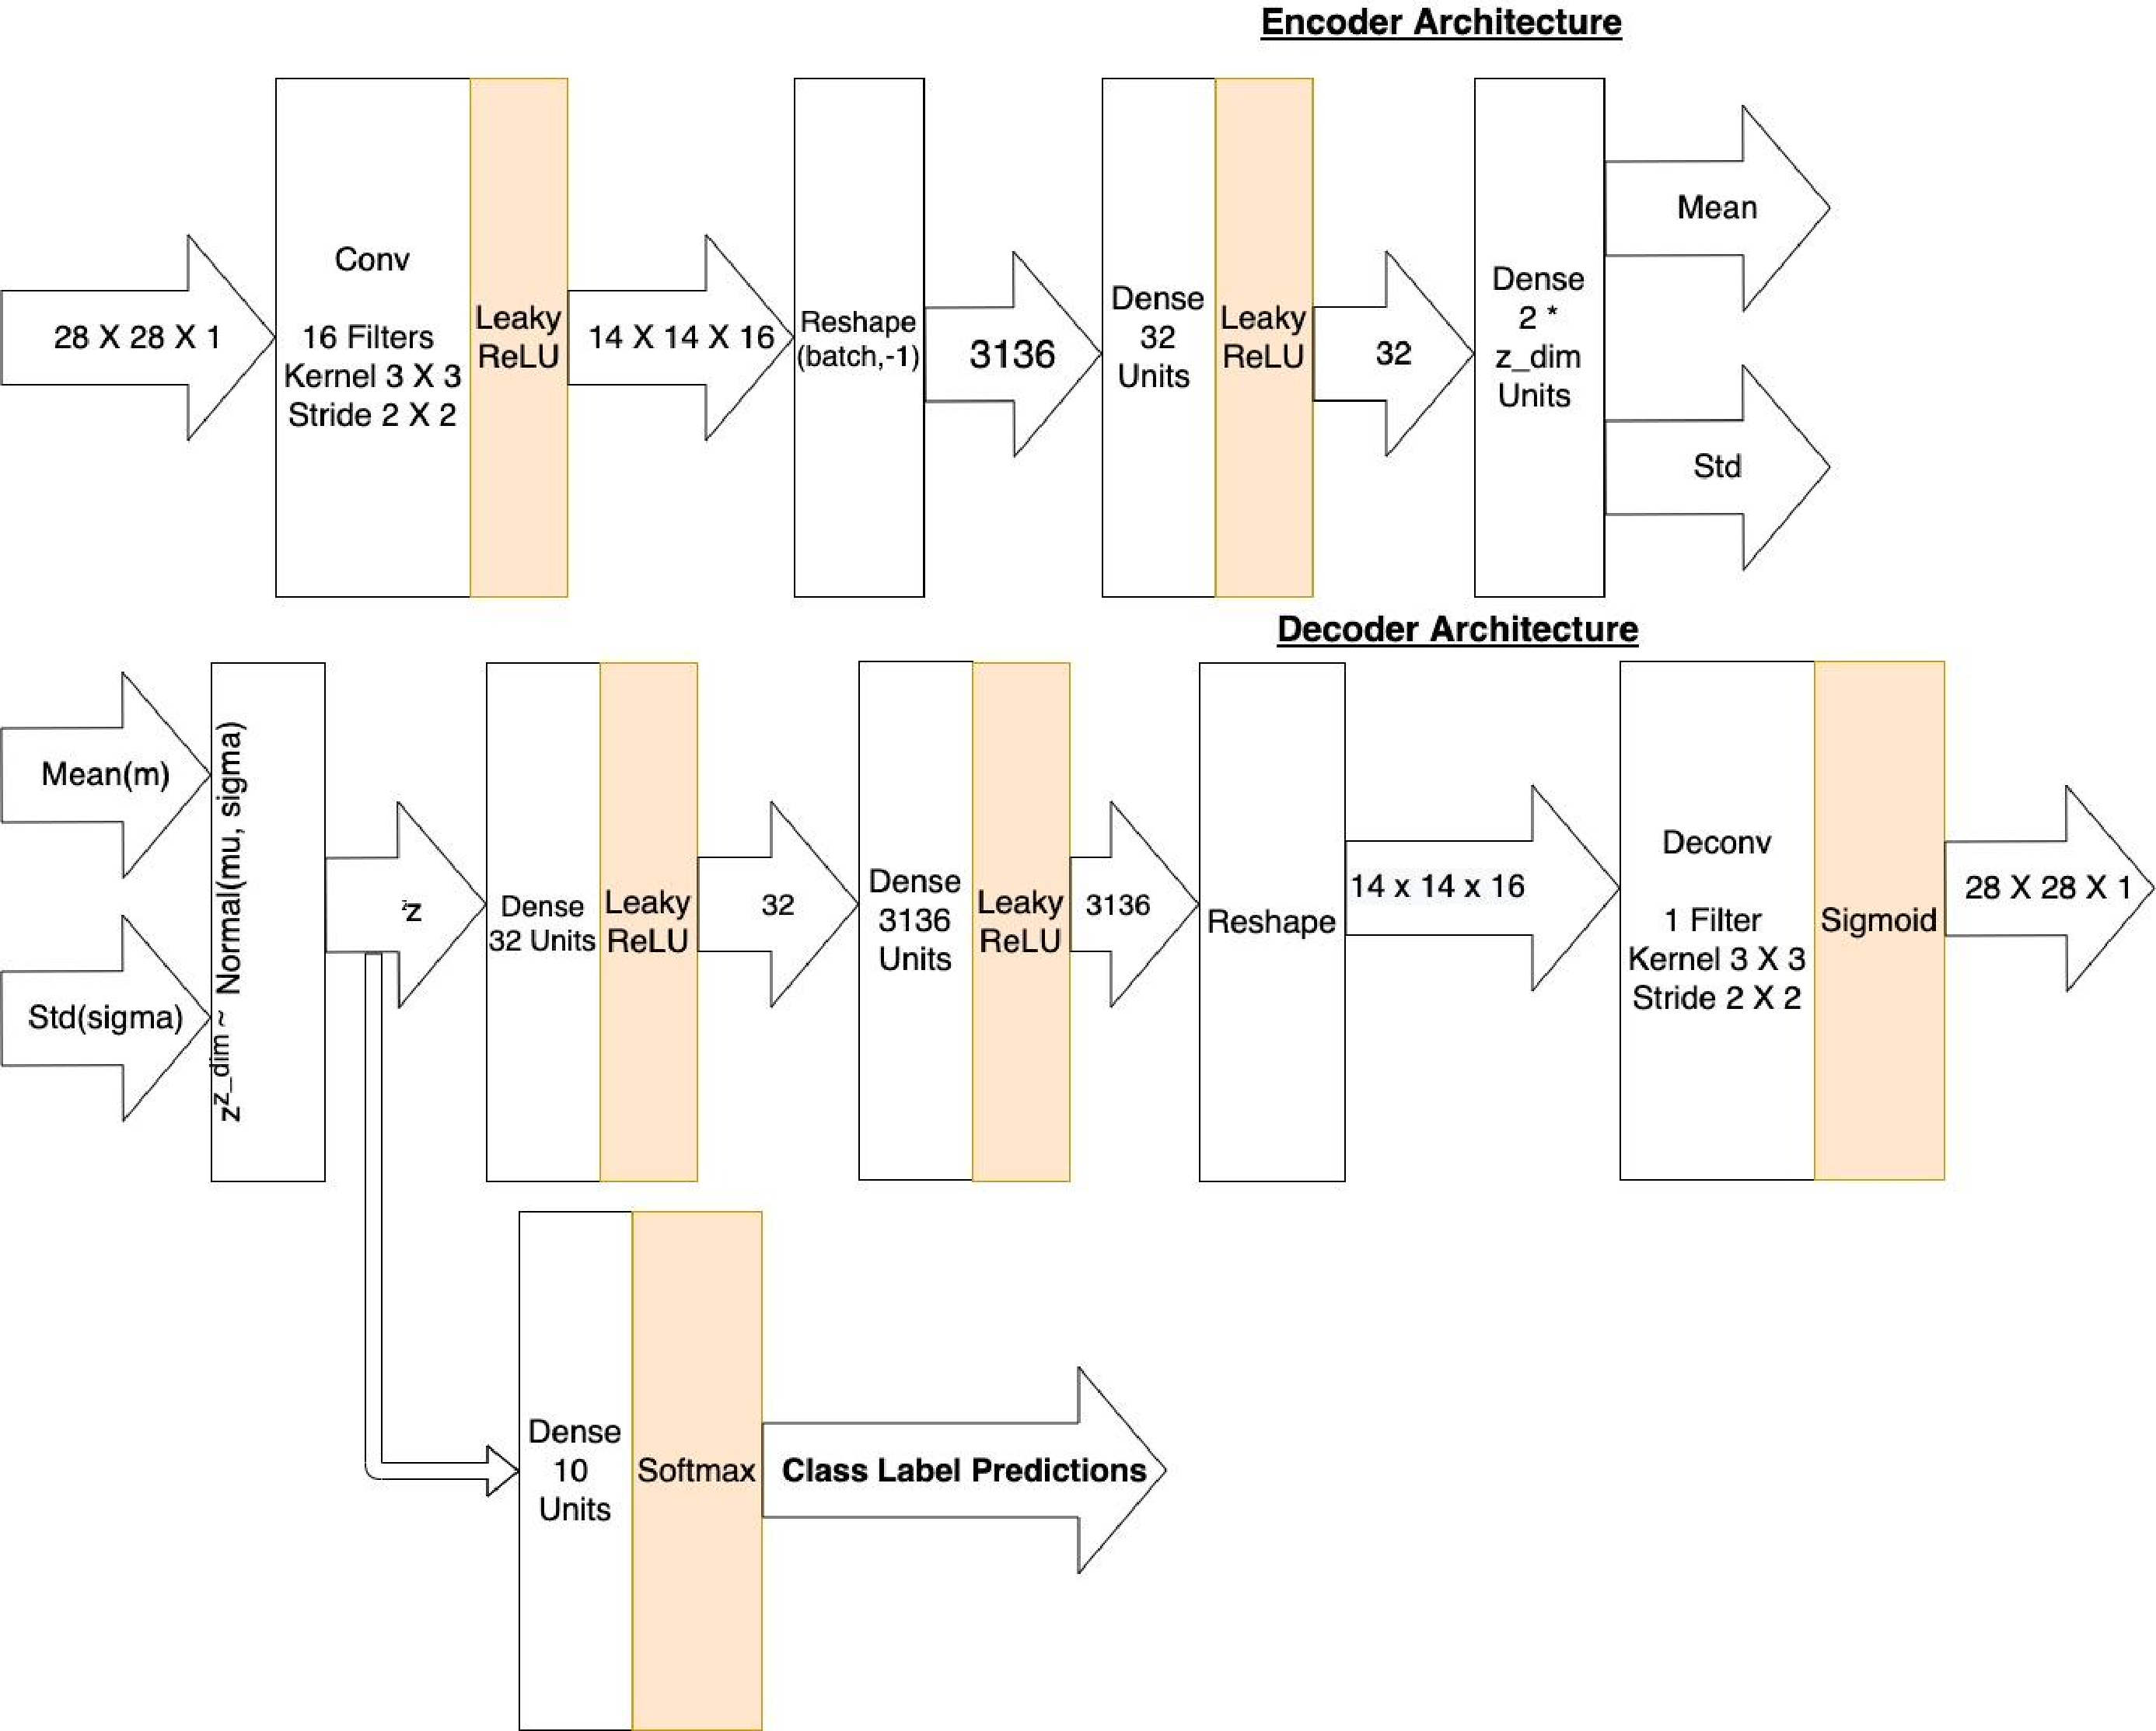
\includegraphics[width=3.5in]{vae_model_architecture_classification_v2}
\DeclareGraphicsExtensions.
\caption{Proposed model architecture}
\label{vae_architecture}
\end{figure}

Figure \ref{vae_architecture} shows the architecture of the proposed model used with MNIST dataset.
The model follows the usual encoder-decoder architecture found in VAE.
The encoder consists of two down-sampling convolutional layers followed by two dense layers.
The decoder is made up of two dense layers and two up-sampling de-convolution layers.
We added an additional softmax classification layer to classify the latent vectors learned by VAE into one of the 10 class labels.

\subsection{Semi-supervised loss function and training}\label{section_loss_function}
The variational autoencoder is initially trained until the reconstruction loss converges using the beta-VAE loss function\cite{beta_vae} given below.

\begin{equation} \label{vae_loss_eqn}
L_{VAE} = -\sum_{i, j}(x_{ij}^n \ln \hat{x}_{ij}^n
+ (1 - x_{ij}^n) \ln(1 -  \hat{x}_{ij}^n ) )\\
    +\beta KLD(p(z), N(0,I))
\end{equation}
where   $x_{ij}$ is the pixel value at position $(i, j)$ of the input image, $\hat{x}_{ij}$ is the pixel value of reconstructed image, $p(z)$ is the probability density function of latent vectors, $N(0,I)$ is the standard multivariate normal distribution of dimension $z_{dim}$ and KLD() deontes KL divergence.
We use binary cross entropy as reconstruction loss for MNIST images, since the output activation function is sigmoid and MNIST images are treated as binary images in our experiments.

Once a reasonably good latent representation is learned using unsupervised $\beta$-VAE loss function mentioned above, the latent vectors corresponding to the training samples are clustered into $k=10$ clusters.
The cluster centers were decoded using the decoder part of VAE and the resulting images corresponding to cluster centers were manually given a label and a confidence.
Figure \ref{cluster_center_1} shows the reconstructed images of cluster centers after unsupervised training.
If the cluster center for a cluster does not correspond to any valid digit image, all the samples in that cluster are again clustered into $k$ clusters and a further attempt is made to label the cluster centers of second level clusters.
The process can be continued to form clusters at multiple levels based on the available manual annotation budget.
The labels assigned to the cluster center is then propagated to all other samples in the cluster using the following strategy
\begin{enumerate}
    \item Each sample in the cluster is assigned with the  same label as the cluster center.
    \item Each sample is also given a confidence based on its distance from cluster center and  a manually assigned confidence in the range of [0,1]. The overall confidence of  training sample $x^n$ is computed as
\begin{equation}
w_n = p_cf(d_n)
\end{equation}
where $d_n$ is the distance of the sample from its cluster center, $p_c$  is the confidence manually assigned to the cluster center and $f: d \mapsto [0,1]$ is a monotonically decreasing function that maps distance to a confidence value in unit interval [0,1].
\end{enumerate}

\begin{figure}
\centering
\begin{minipage}{.5\textwidth}
  \centering
  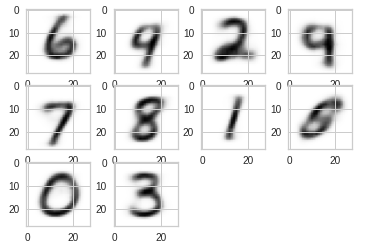
\includegraphics[width=.9\linewidth]{cluster_centers_epoch_1_0_gmm.png} \\
  \captionof{figure}{Cluster centers after unsupervised training}
  \label{cluster_center_1}
\end{minipage}%
\begin{minipage}{.5\textwidth}
  \centering
  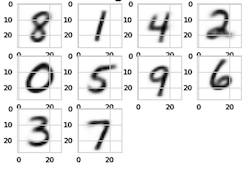
\includegraphics[width=.9\linewidth]{cluster_centers_epoch_5_0_gmm.png} \\
  \captionof{figure}{Cluster centers after 5 iterations of semi-supervised training}
  \label{cluster_center_5}
\end{minipage}
%\label{cluster_center}
\end{figure}

Experiments were performed with different choices for the distance metric(Euclidean and Mahalanobis) and confidence decay function $f$.
For the confidence decay function, we tried both the exponential decay function and one-sided Gaussian function as given in equation \ref{exp_decay} and \ref{gaussian_decay} respectively.
\begin{equation}
    w_n = p_ce^{-a d_n}
    \label{exp_decay}
\end{equation}

\begin{equation}
    w_n = p_ce^{-a d_n^2}
    \label{gaussian_decay}
\end{equation}
where $a$ is a hyper parameter determining how fast the confidence decreases with the distance from cluster center.


Training is continued for more epochs using the modified loss function, given below, that incorporates the manual labels and confidence into account.
\begin{equation} \label{semi_supervised_loss}
L = L_{VAE}  - \gamma \sum_{k=0}^{K}w_{n}y_{nk}\ln(\hat{y}_{nk})
\end{equation}

where $y_{nk}$ is the one-hot encoded label and $\hat{y}_{nk}$ is the predicted softmax probability.
The new term added to the loss is the weighted multi-class cross entropy loss for classification task.


We also performed experiments by using GMM instead of k-means for clustering.
When using GMM for clustering we directly used the product of posterior probability of the sample and cluster center confidence $p_c$ as the overall sample confidence.

As expected we obtained the best performance with Gaussian mixture model.
It is also observed that when k-means is used the Mahalanobis distance along with a Gaussian confidence decay function gave the better result as opposed to Euclidean distance with exponential function.
\section{Experiments}
In order to choose the optimum choice for hyper-parameters like clustering algorithm, distance metric and confidence decay function, we ran semi-supervised experiments on MNIST images for 5 iterations with different combinations of hyper parameters.

\section{Results and Discussions}
\begin{figure}
\centering
\begin{minipage}{.5\textwidth}
  \centering
  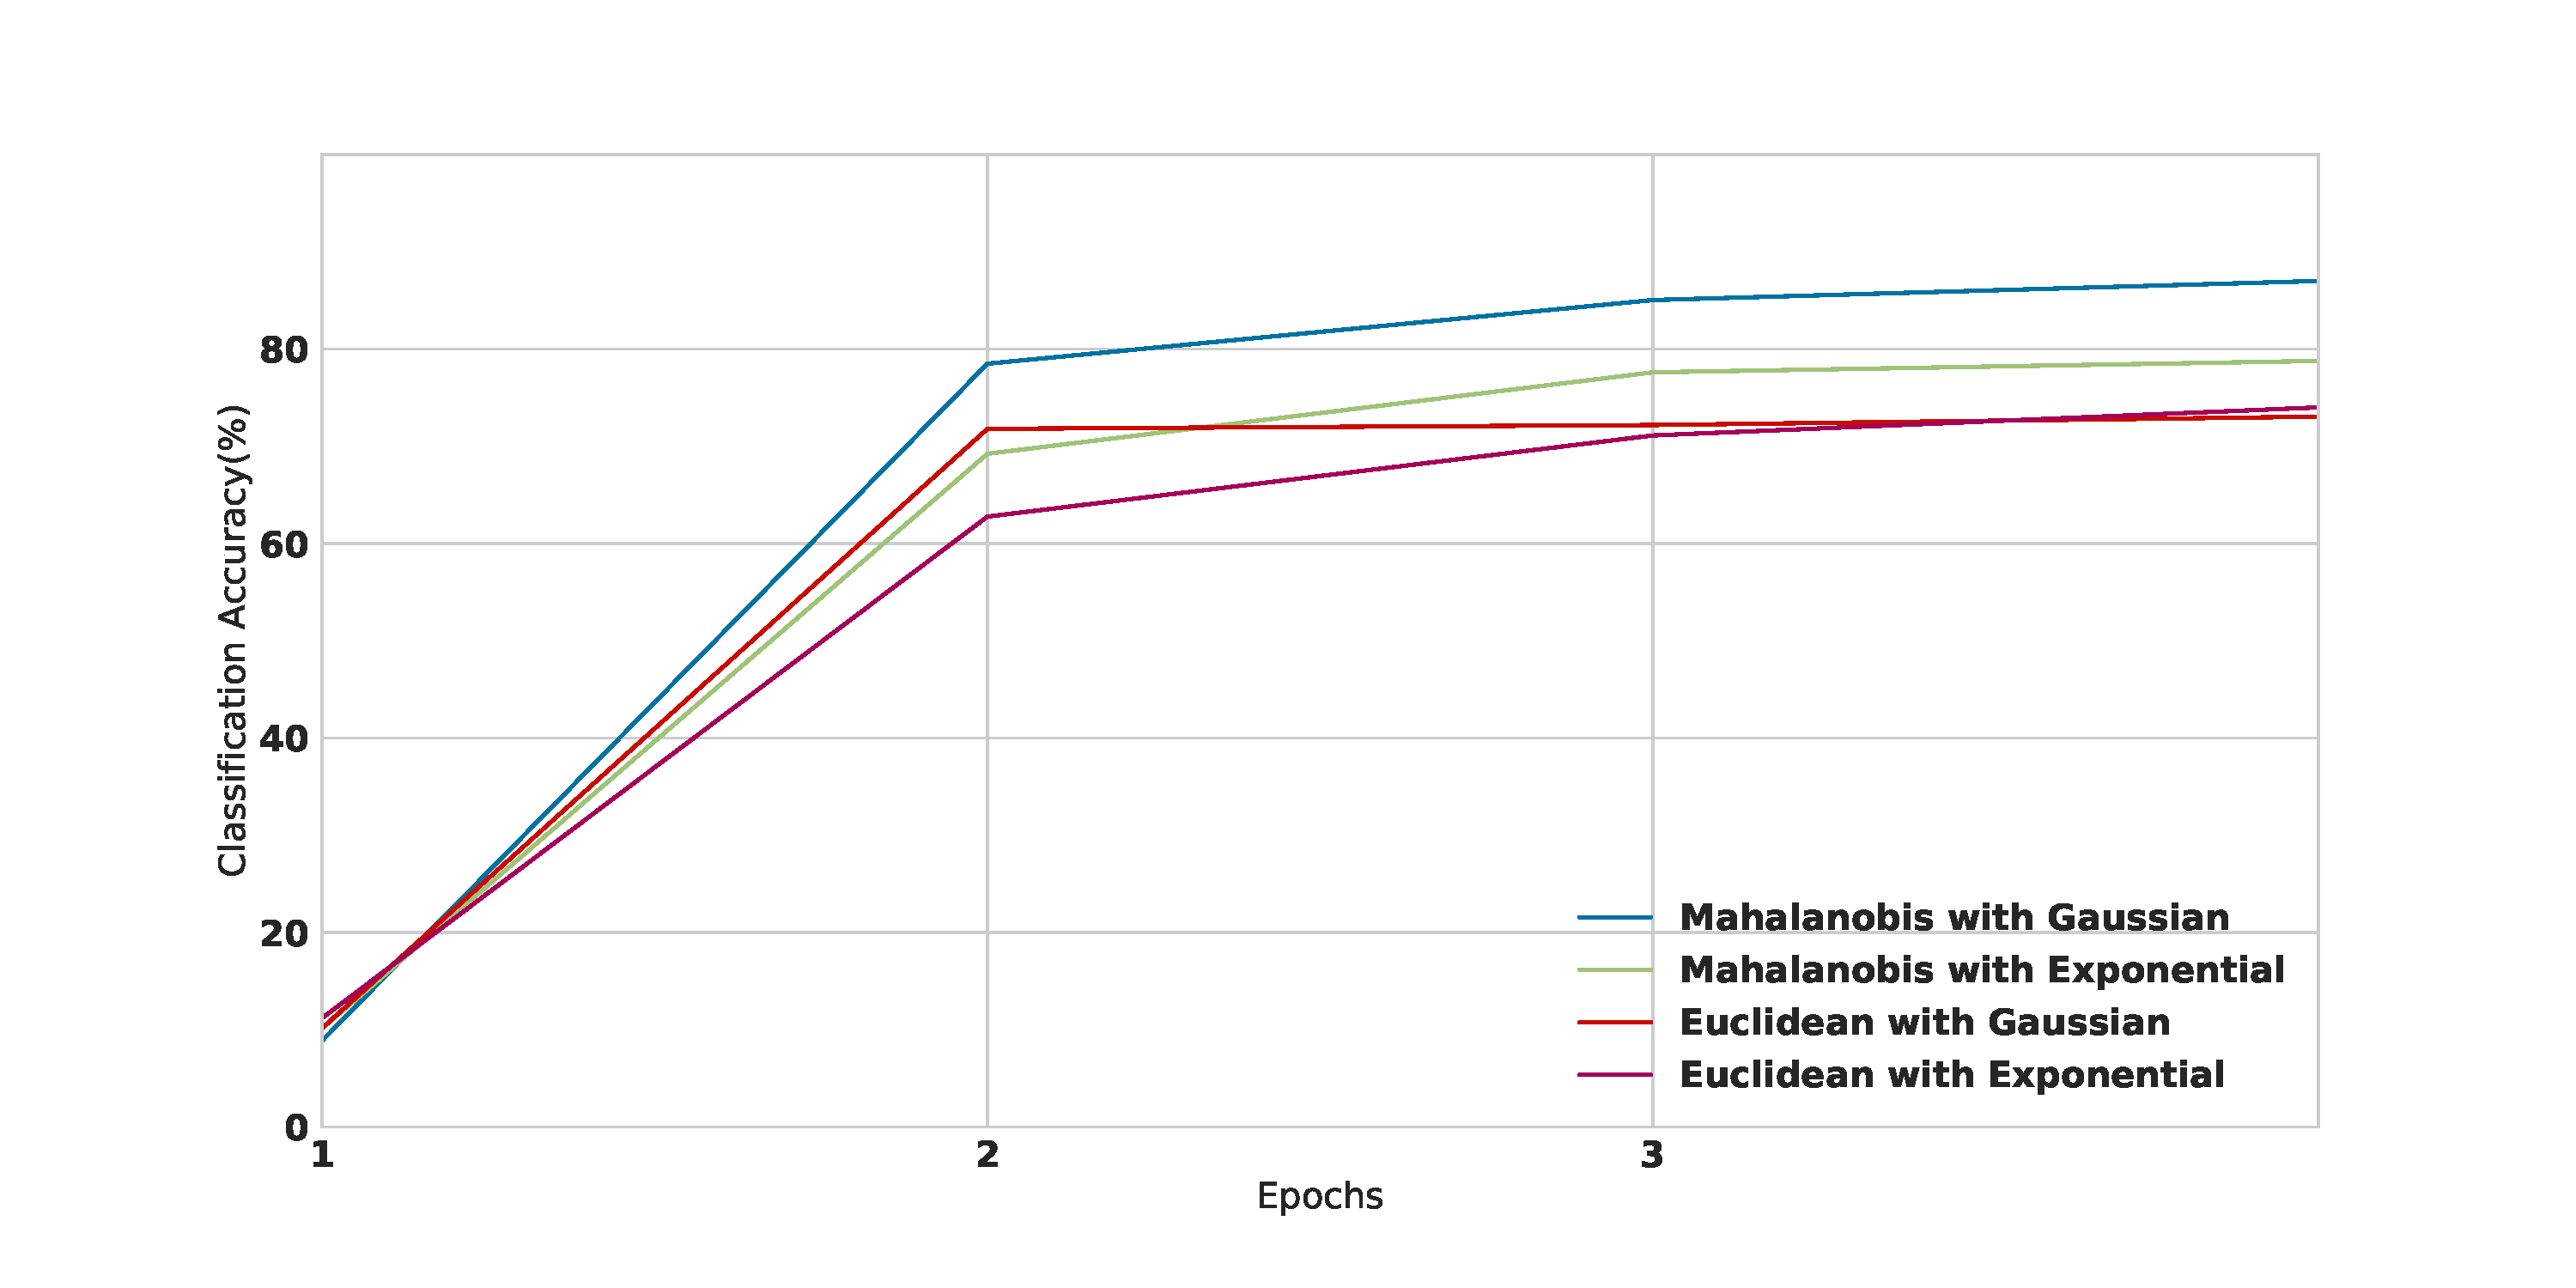
\includegraphics[width=.9\linewidth]{classification_accuracy_hyperparameter}
  \captionof{figure}{Comparison of model performance using k-means}
  \label{classification_acc_hyper_parameter}
\end{minipage}%
\begin{minipage}{.5\textwidth}
  \centering
  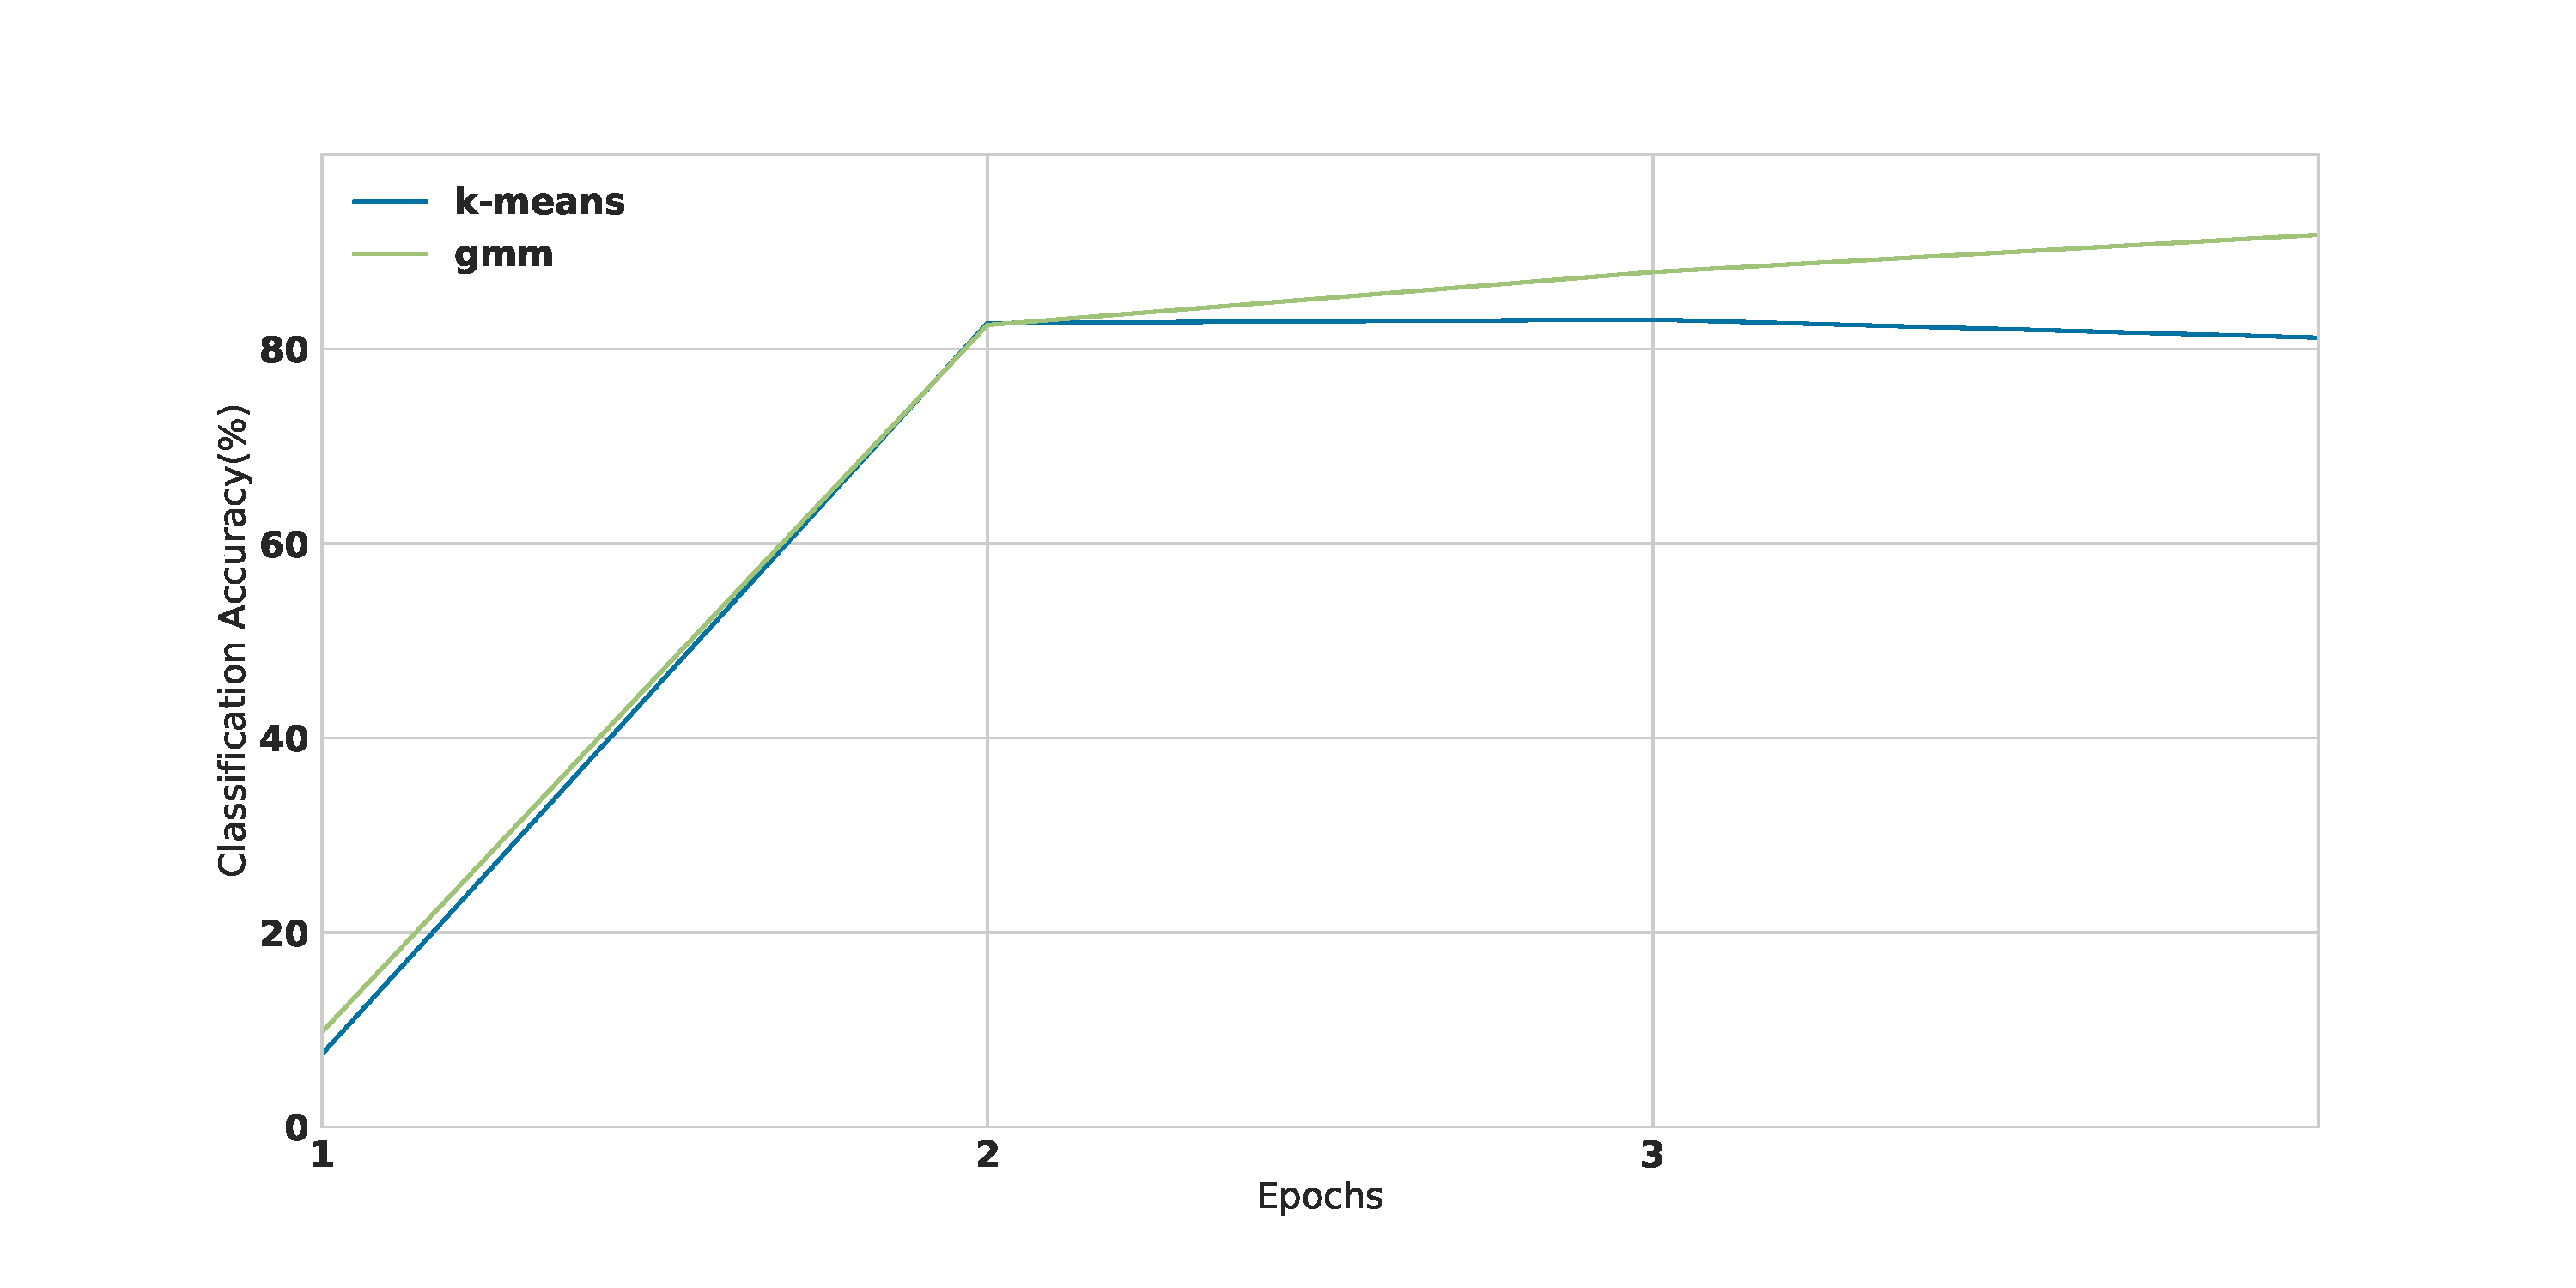
\includegraphics[width=.9\linewidth]{classification_accuracy_kmeans_gmm}
  \captionof{figure}{Comparison of model performance k-means vs gmm}
  \label{classification_acc_kmeans_gmm}
\end{minipage}
%\label{classification_acc}
%    \caption{Classification accuracy}
\end{figure}


Figures \ref{classification_acc_hyper_parameter} shows comparison of classification accuracy when k-means algorithm is used for clustering  with different choices for distance metric and confidence function.
Performance is better when a one-sided Gaussian curve is used as distance-to-confidence mapping function, as opposed to an exponentially decaying function.
This is expected as exponential function decreases at a faster rate near zero.
Hence, the confidence for samples closer to the cluster center decreases at a faster rate as one moves away from cluster center.
Whereas  with Gaussian confidence function, since the gradient of the curve is zero when the argument is near zero, all samples closer to the cluster center will have same confidence as the cluster center confidence $p_c$ which is a desired behaviour.
Another observation is that performance is higher when using Mahalanobis distance instead of Euclidean distance.
This is because the clusters in latent dimensions for each digit have different variance along different direction.
Figure \ref{classification_acc_kmeans_gmm} shows comparison of classification accuracy using k-means and GMM algorithms.
The Gaussian mixture model performs better as the clusters are formed using Mahalanobis distance and the posterior probability is also based on the Mahalanobis distance.
GMM clustering were chosen for all the subsequent experiments.

The reconstructed images of cluster centers shown in Figure \ref{cluster_center_1} and Figure \ref{cluster_center_5} shows that as training progresses, the clusters formed in latent space correspond to different classes in MNIST dataset.
In Figure \ref{cluster_center_1} some of the cluster center does not correspond to any valid digit, and some digits like 4  are missing.
A further investigation revealed that this is happening because the latent vectors for samples 4 and 9 were very similar and got clustered into the same cluster.
However, after a few epochs of training with classification loss added, the latent vector for symbol 9 and 4 is getting clustered into different clusters as is evident from Figure \ref{cluster_center_5}.
This is also evident from the tsne visualization of latent vectors corresponding to symbols 4 and 9  shown in Fig \ref{tsne_un_4_9} and Figure \ref{tsne_semi_4_9}.

Figure \ref{tsne_un} and Figure \ref{tsne_semi} shows the 2-d tsne visualization of the latent vector distribution for the entire training set with unsupervised and semi-supervised training.
As evident from this figure, the distribution of samples from different classes become more separable with the introduction of classification loss.

Figure \ref{classification_acc_unsupervised} shows the  classification accuracy on test dataset during the initial 10 epochs of training.
It is observed that the classification accuracy increases by about $3\%$ even without using any labelled data.
From this it is evident that as the unsupervised VAE training progresses the classification accuracy also increases.
However, the increase in classification accuracy is very slow.
After epoch $10$ the semi-supervised mode of training was started.
Fig \ref{classification_acc_semi_supervised}  shows the increase in classification accuracy along with the number of samples annotated  during semi-supervised training mode.


\begin{figure}
\centering
\begin{minipage}{.5\textwidth}
  \centering
  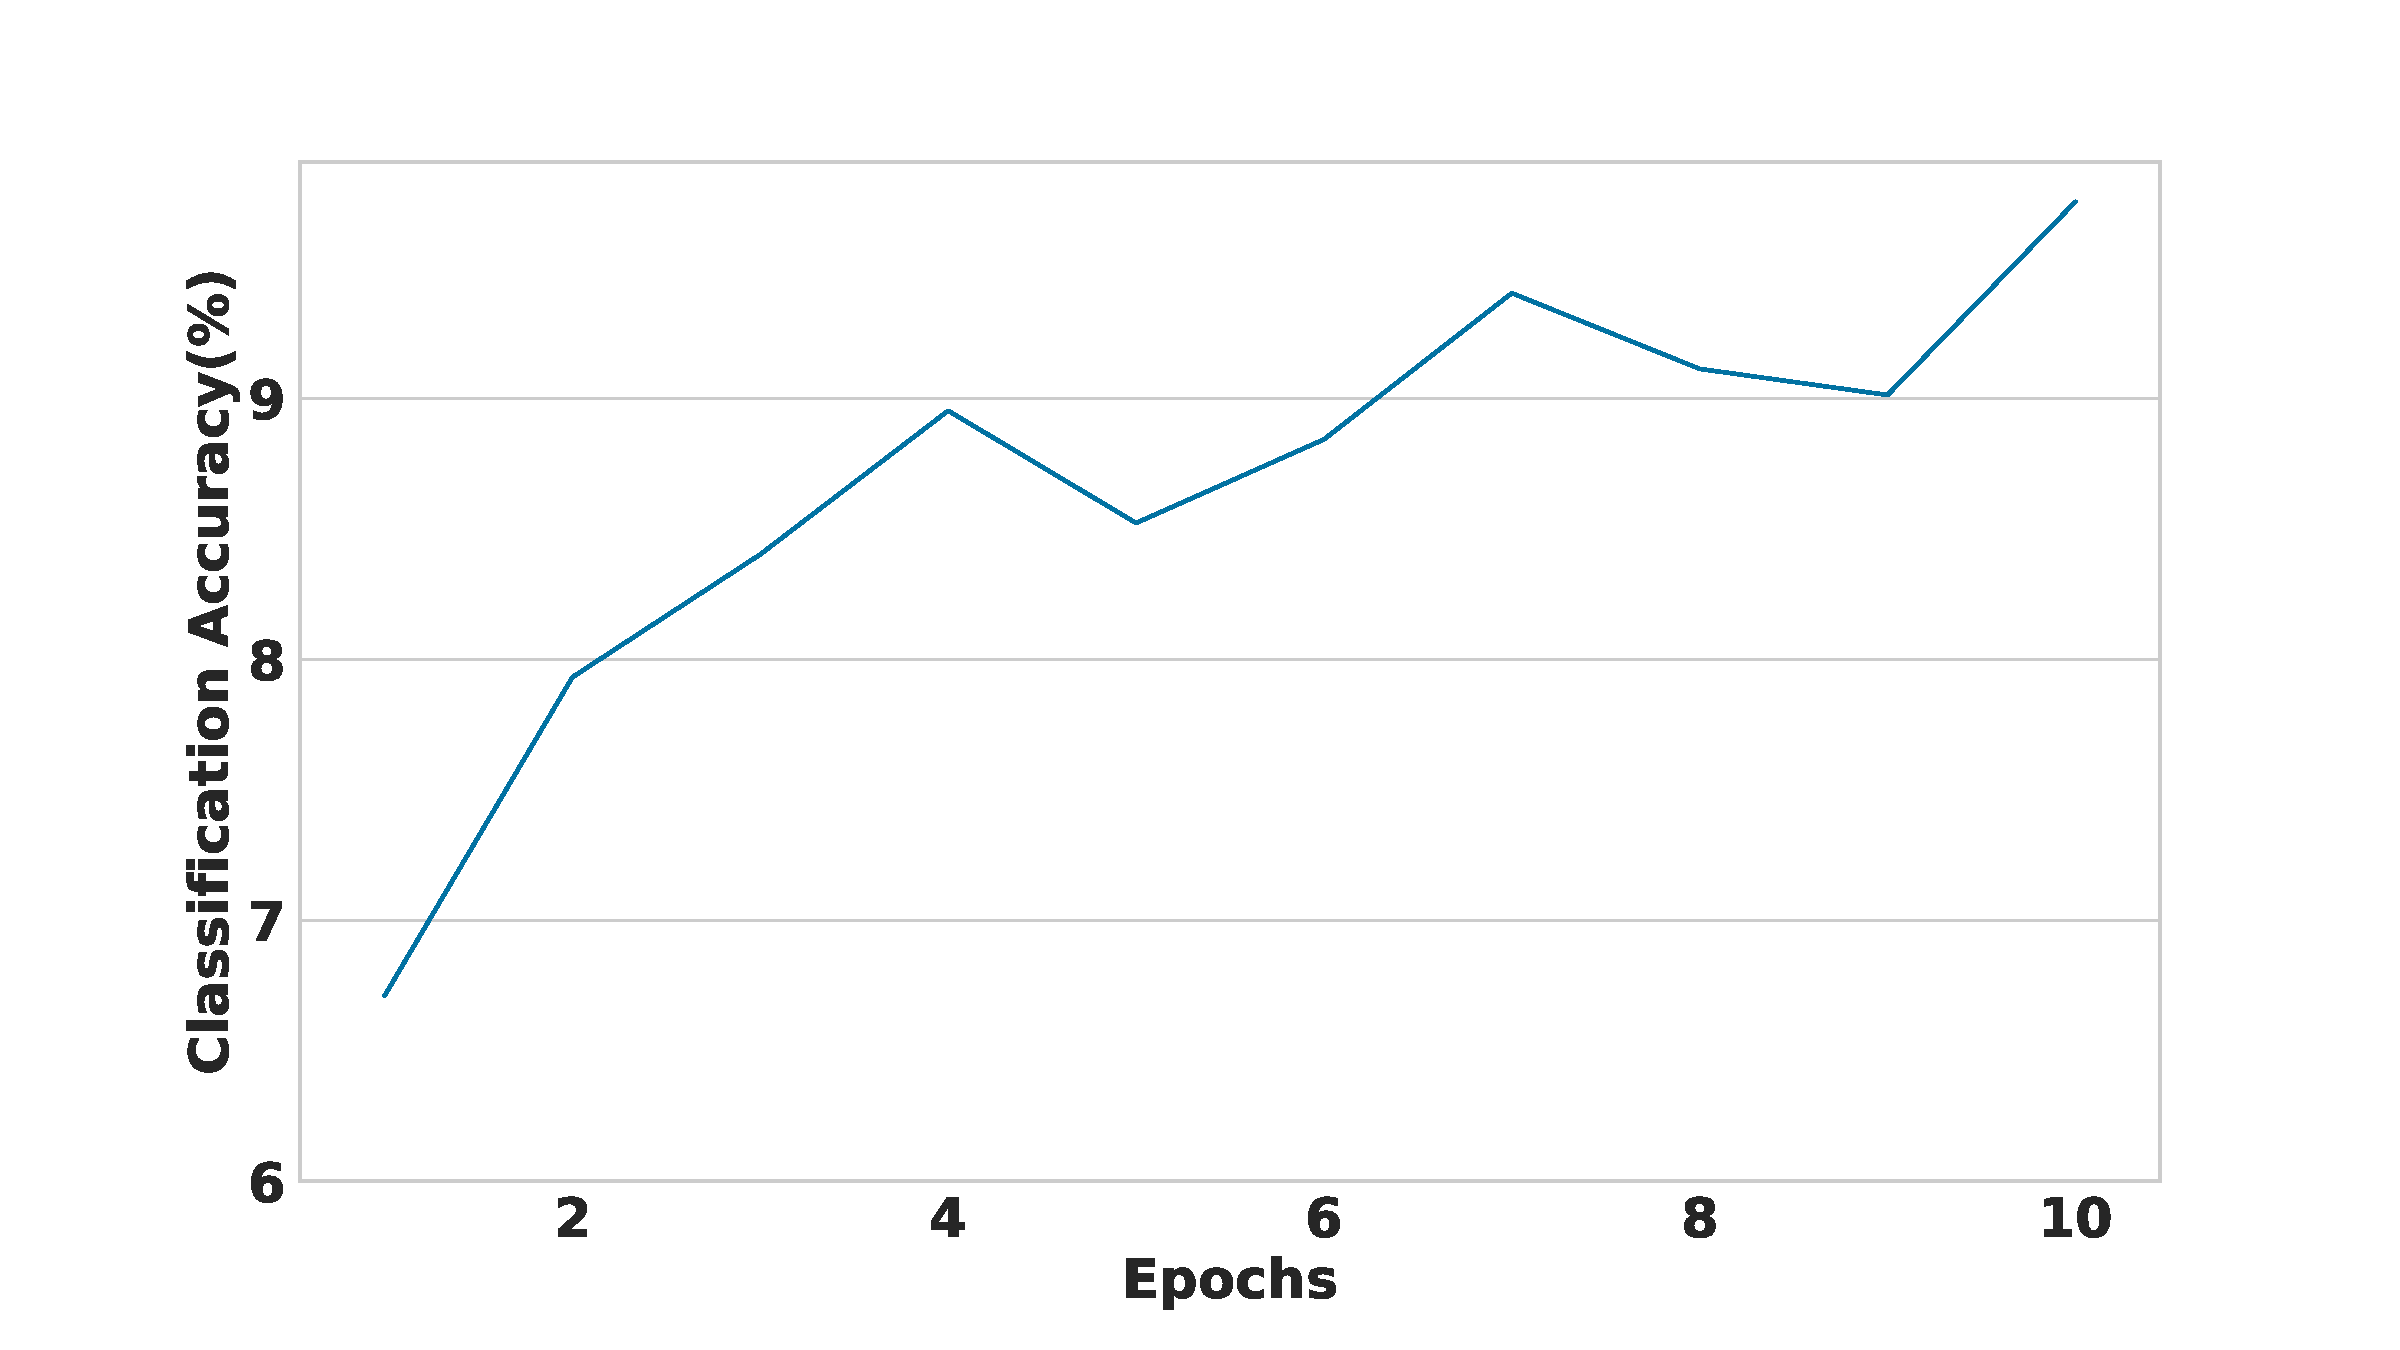
\includegraphics[width=.9\linewidth]{classification_acc_unsupervised}
  \captionof{figure}{Unsupervised training}
  \label{classification_acc_unsupervised}
\end{minipage}%
\begin{minipage}{.5\textwidth}
  \centering
  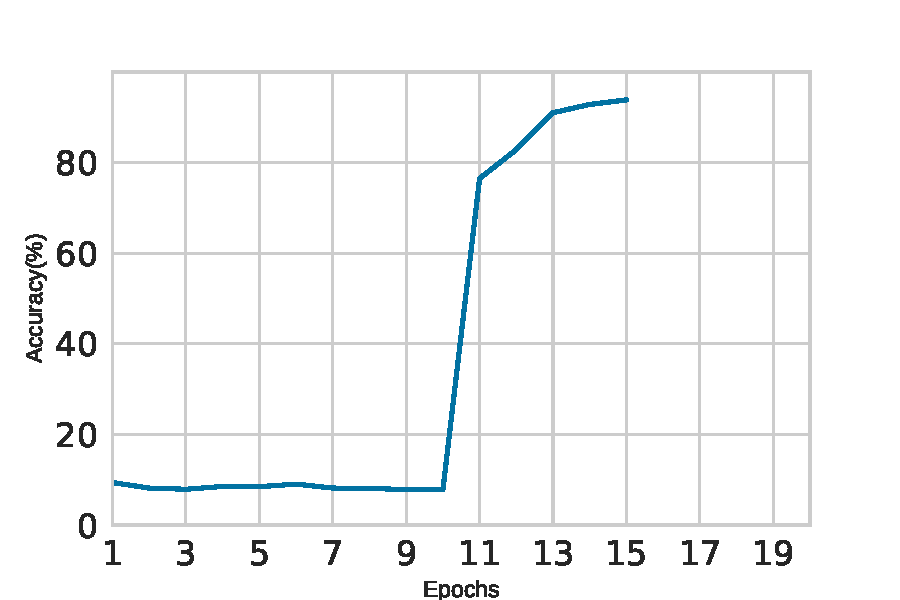
\includegraphics[width=.9\linewidth]{classification_acc_semi_supervised}
  \captionof{figure}{Semi-supervised training started after 10 epochs.}
  \label{classification_acc_semi_supervised}
\end{minipage}
%    \label{classificaion_acc}
%    \caption{Classification accuracy}
\end{figure}

\begin{figure}
\centering
\begin{minipage}{.5\textwidth}
  \centering
  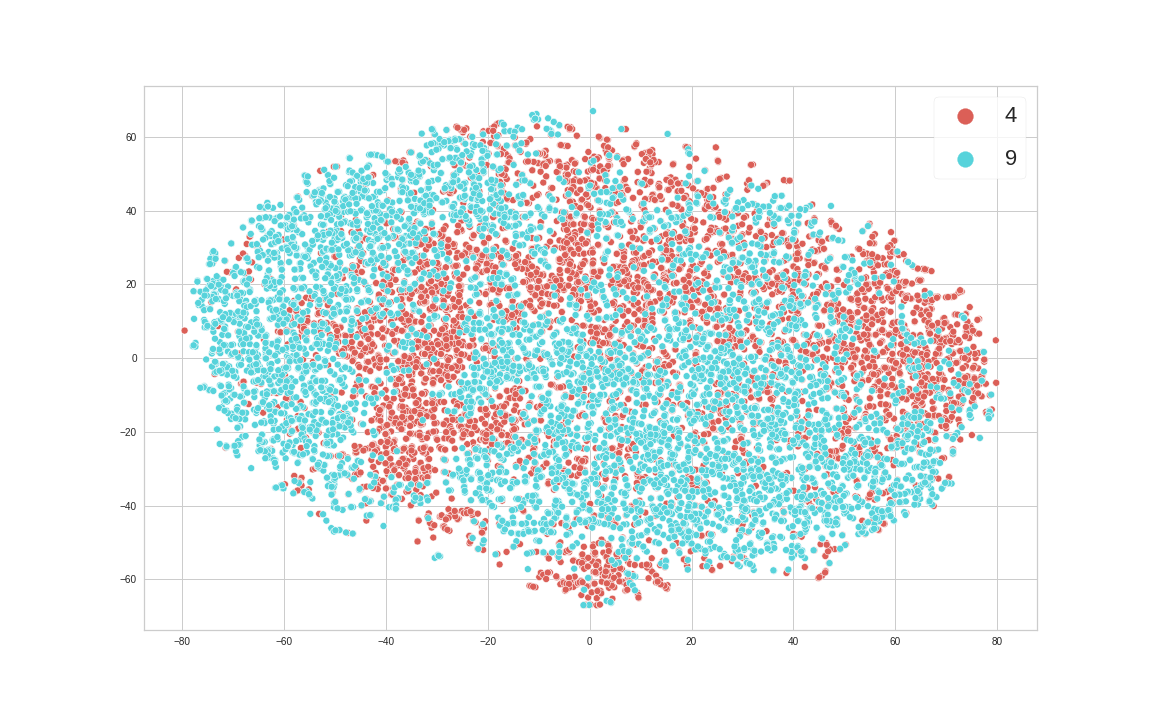
\includegraphics[width=.9\linewidth]{tsne_4_9_unsup.png}
  \captionof{figure}{Unsupervised}
  \label{tsne_un_4_9}
\end{minipage}%
\begin{minipage}{.5\textwidth}
  \centering
  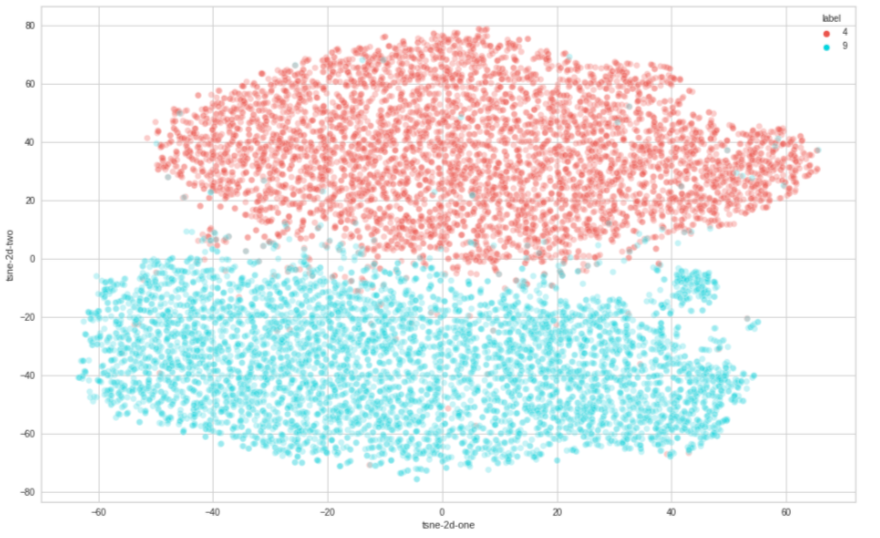
\includegraphics[width=.9\linewidth]{tsne_4_9_semi.png}
  \captionof{figure}{Semi-supervised}
  \label{tsne_semi_4_9}
\end{minipage}
%    \label{tsne}
%    \caption{2-d tsne visualization of learned latent space distribution}
\end{figure}


\begin{figure}
\centering
\begin{minipage}{.5\textwidth}
  \centering
  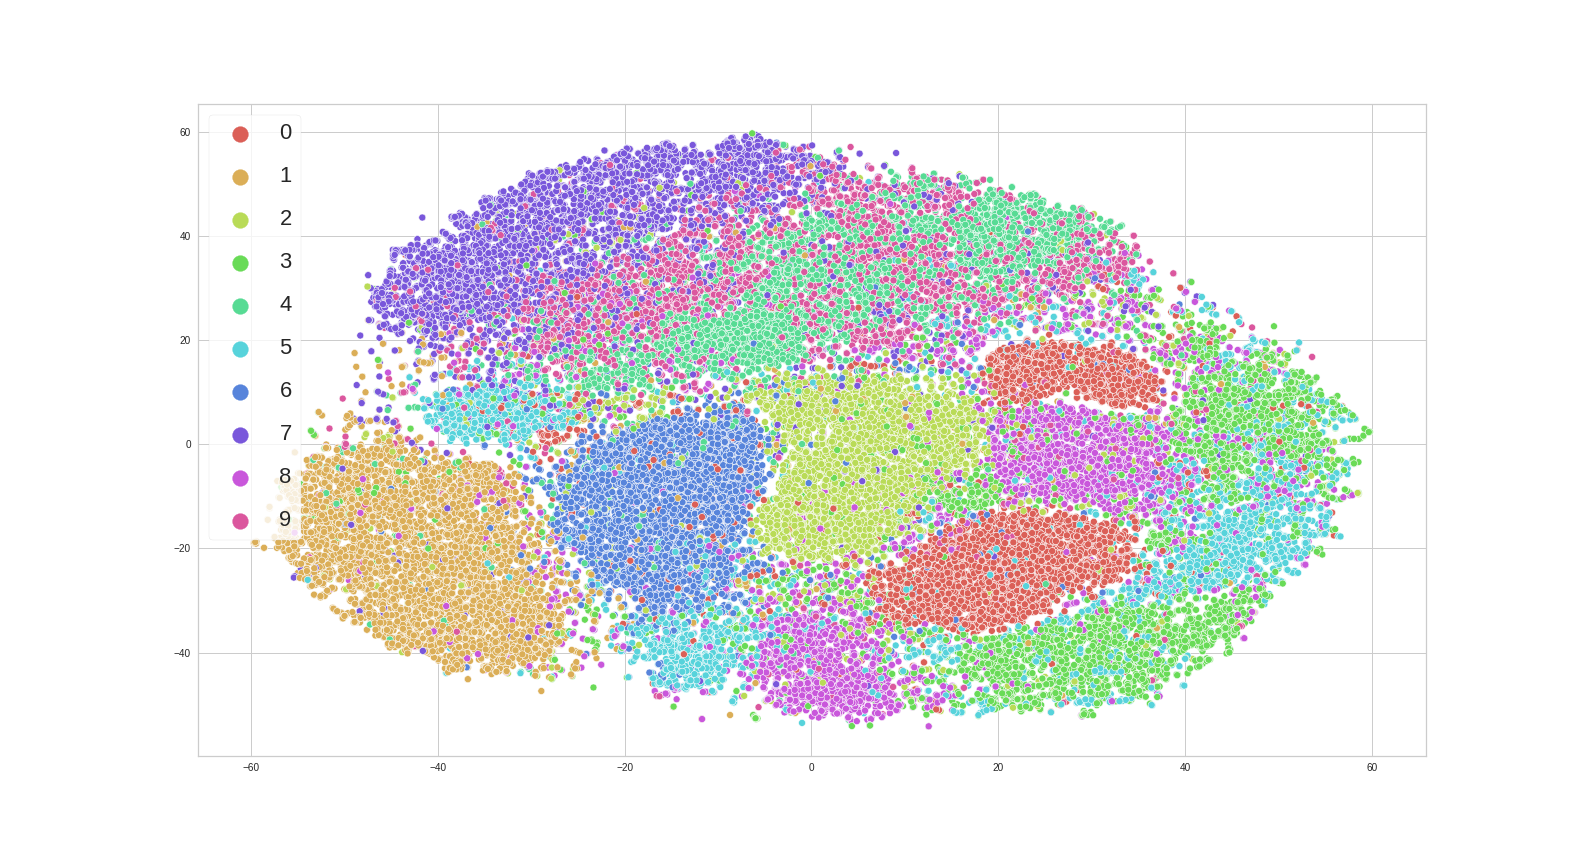
\includegraphics[width=.9\linewidth]{tsne_unsup.png}
  \captionof{figure}{Unsupervised}
  \label{tsne_un}
\end{minipage}%
\begin{minipage}{.5\textwidth}
  \centering
  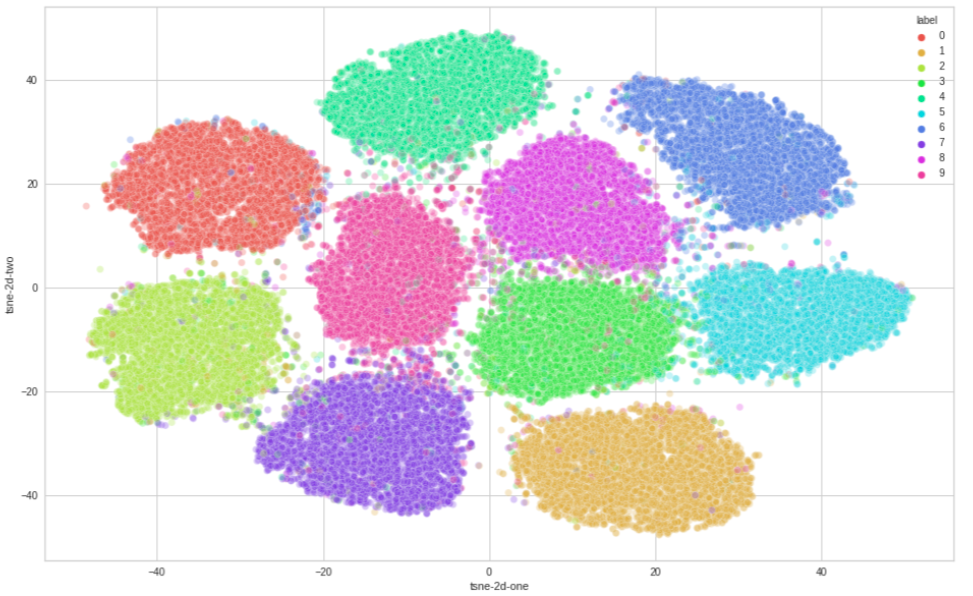
\includegraphics[width=.9\linewidth]{tsne_semi.png}
  \captionof{figure}{Semi-supervised}
  \label{tsne_semi}
\end{minipage}
%    \label{tsne}
%    \caption{2-d tsne visualization of learned latent space distribution}
\end{figure}


\section{Conclusion}
%
% ---- Bibliography ----
%
% BibTeX users should specify bibliography style 'splncs04'.
% References will then be sorted and formatted in the correct style.
%
\bibliographystyle{splncs04}
\bibliography{mybibliography}
%
\begin{thebibliography}{8}
    \bibitem{alexnet}
    Krizhevsky, Alex, Ilya Sutskever, and Geoffrey E. Hinton. Imagenet classification with deep convolutional neural networks. Advances in neural information processing systems 25 (2012): 1097-1105
    \bibitem{vggnet}
    Simonyan, Karen, and Andrew Zisserman. Very deep convolutional networks for large-scale image recognition. arXiv preprint arXiv:1409.1556 (2014)
    \bibitem{resnet}
    He, Kaiming, et al. Deep residual learning for image recognition. Proceedings of the IEEE conference on computer vision and pattern recognition. 2016.
    \bibitem{deeplab}
    Chen, Liang-Chieh, et al. Deeplab: Semantic image segmentation with deep convolutional nets, atrous convolution, and fully connected crfs. IEEE transactions on pattern analysis and machine intelligence 40.4 (2017): 834-848.
    \bibitem{unet}
    Ronneberger, Olaf, Philipp Fischer, and Thomas Brox. U-net: Convolutional networks for biomedical image segmentation. International Conference on Medical image computing and computer-assisted intervention. Springer, Cham, 2015.
    \bibitem{yolo}
    Redmon, Joseph, et al. You only look once: Unified, real-time object detection. Proceedings of the IEEE conference on computer vision and pattern recognition. 2016.
    \bibitem{faster_rcnn}
    Ren, Shaoqing, et al. Faster r-cnn: Towards real-time object detection with region proposal networks. arXiv preprint arXiv:1506.01497 (2015).
    \bibitem{beta_vae}
    Higgins, Irina, et al. beta-vae: Learning basic visual concepts with a constrained variational framework. (2016)

    \bibitem{kingma_2014}
    Kingma, Diederik P., et al. Semi-supervised learning with deep generative models. arXiv preprint arXiv:1406.5298 (2014)

    \bibitem{vaal}
    Sinha, Samarth, Sayna Ebrahimi, and Trevor Darrell. Variational adversarial active learning. Proceedings of the IEEE/CVF International Conference on Computer Vision. 2019
    \bibitem{vae}
    Kingma, Diederik P., and Max Welling. Auto-encoding variational bayes. arXiv preprint arXiv:1312.6114 (2013).
    \bibitem{gan}
    Goodfellow, Ian J., et al. Generative adversarial networks. arXiv preprint arXiv:1406.2661 (2014).
    \bibitem{mahapatra_2018}
    Mahapatra, Dwarikanath, et al. Efficient active learning for image classification and segmentation using a sample selection and conditional generative adversarial network. International Conference on Medical Image Computing and Computer-Assisted Intervention. Springer, Cham, 2018.
    \bibitem{mayer_2020}
    Mayer, Christoph, and Radu Timofte. Adversarial sampling for active learning. Proceedings of the IEEE/CVF Winter Conference on Applications of Computer Vision. 2020.
    \bibitem{wang_2016}
    Wang, Keze, et al. Cost-effective active learning for deep image classification. IEEE Transactions on Circuits and Systems for Video Technology 27.12 (2016): 2591-2600.
    \bibitem{beluch_2018}
    Beluch, William H., et al. The power of ensembles for active learning in image classification. Proceedings of the IEEE Conference on Computer Vision and Pattern Recognition. 2018.
\end{thebibliography}
\end{document}
